\chapter{Caracterización de la madera de palmera en ultrasonidos}

El interés de la madera como material de construcción, o materia prima para
la fabricación de herramientas, instrumentos musicales, mobiliario o
carpintería naval ---por citar algunos ejemplos de la multitud de usos que
recibe la madera en la actualidad--- ha originado desde principios de siglo
un interés por el estudio de sus propiedades físicas. Recientemente los
ensayos no destructivos por ultrasonidos han tenido un papel importante en
el estudio de las características estructurales de la madera, especialmente
en la detección de discontinuidades como grietas, presencia de
acebolladuras o nudos. El interés por las propiedades estructurales de la
madera se justifica asimismo puesto que en muchas de sus aplicaciones de su
integridad depende la seguridad de sus usuarios, viendo como ejemplo más
claro de ello el uso de madera en la construcción.

Además, existe un interés patente por otras propiedades de la madera, como
sus propiedades mecánicas, al conocer las propiedades mecánicas de
distintos tipos de madera en distintas circunstancias es posible determinar
el mejor uso para cada tipo; o acústicas, la madera es útil en la creación
de cavidades resonantes o como aislante acústico pues muestra una alta
capacidad para atenuar el ruido. Los \sig{endus} han demostrado ser un
método efectivo para determinar las propiedades mecánicas y acústicas de la
madera.

Las palmeras, aunque también útiles para la construcción por sus
propiedades (al ser una madera blanda y ligera, la madera palmera se
utiliza sobre todo en la construcción de tejados y tejadillos), han pasado
a ser un importante elemento decorativo en los núcleos urbanos, e incluso
en ciertas localizaciones constituyen un elemento importante del patrimonio
cultural y medioambiental.

Como parte de la decoración urbana la palmera está sometida a la acción de
un medio hostil, en el que se dan grandes temperaturas y en el que sufre la
acción de agentes externos que en otros entornos no existen o muestran
menor actividad. Como género de plantas apreciado, existe un interés por
saber como afecta a la palmera su entorno, conocimiento que puede
alcanzarse contrastando las propiedades físicas de la madera de palmera
cuando está sujeta a la acción de distintos medios. Así mismo, la madera de
palmera defectuosa también puede ser causa de accidentes ---por ejemplo,
los jardineros debe subirse a las copas de las palmeras para su
mantenimiento, las palmeras que presentan deficiencias estructurales
constituyen un riesgo para su integridad física--- por lo que el
conocimiento de las características estructurales de un ejemplar,
especialmente de los ejemplares in vivo, adquiere vital importancia. Las
aplicaciones basadas en ultrasonidos parecen especialmente adecuadas al
tratar de deducir las propiedades físicas de palmeras vivas, pues cuentan
con la ventaja de no dañar el ejemplar.


\section{Objetivos del experimento}

La madera de palmera es desde el punto de vista de su estudio como medio de
propagación acústico dentro del conjunto de las distintas maderas cuanto
menos un medio peculiar podría decirse incluso, sin temor a equivocarse,
que es atípico. Ello se debe a las características propias del género; la
palmera, a pesar de ser una planta de tipo arbustivo crece ---la mayor
parte de las veces motivada por la acción del ser humano--- en forma
arborescente.

Ello se debe a las características propias del género, la palmera, a pesar
de su crecimiento en forma arborescente ---la mayor parte de las veces
motivado por la acción del ser humano--- es una planta de tipo arbustivo.
Es por ello que su tallo a pesar de ser leñoso muestra una composición
distinta a la madera de los árboles, no presenta madera secundaria pues sus
fibras no conservan procambium\footnote{Las fibras o haces vasculares de
las palmeras se denominan colaterales cerrados debido a esta propiedad. En
realidad, el tallo de una palmera es leñoso debido a que contiene
esclerénquima fibroso xilemático, un tejido celular elástico que le sirve
de sostén.} (tejido celular presente en los árboles responsable de su
crecimiento) con lo que carece de verdadero tronco.

De cara a su estudio, el tallo de una palmera presenta una estela (sección
transversal) en la que los haces vasculares formados en su mayor parte por
fibras xilemáticas y vasos liberianos (aquellos que transportan nutrientes
desde la parte autótrofa de la planta a sus partes basales subterráneas) no
se agrupan en ninguna estructura reconocible, si no que están dispersos
formando espacios entre sí rellenos con material blando y húmedo, y aire.
La gran proporción de humedad, el espacio vacío, y la distribución
heterogénea de las fibras dificulta enormemente la propagación de ondas de
media y alta frecuencia a través de un tallo de palmera, algo que no ocurre
en otros tipos de madera.

Actualmente existen muy pocas referencias bibliográficas que documenten que
tipo de información, parámetros o propiedades físicas pueden extraerse de
un ensayo por ultrasonidos en madera de palmera. En general, es muy difícil
encontrar información que relacione los parámetros físicos deducibles
mediante técnicas no destructivas basadas en ultrasonidos y las
características microestructurales inducidas por condiciones adversas en
madera de palmera. Menos aún si se trata de ensayos realizados con
transductores de impacto, pruebas realizadas con esta tecnología son muy
escasas.

Al disponer en el laboratorio de unos transductores de impacto,
recientemente obtenidos, se plantea como parte del proyecto fin de carrera
la realización de un estudio preliminar cuyos resultados puedan justificar
el interés en abordar un proyecto mucho más ambicioso en este campo. Cabe
remarcar aquí que como estudio preliminar este apartado del proyecto no
pretende aportar más que una serie de resultados que deberán valorarse
única y exclusivamente con el propósito aquí especificado.


\subsection{Elección de bajas frecuencias}

Es bien sabido (y se expone con detalle en el \vref{chap:endus} de esta
memoria) que las ondas ultrasónicas presentan un comportamiento variable
con respecto a la frecuencia. En este subapartado se justifica la elección
de las bajas frecuencias para el desarrollo de esta aplicación poniendo de
manifiesto cuales son las ventajas y desventajas que presentan en este tipo
de ensayos.


\subsubsection{Ventajas}

Como se observó en el capítulo anterior, uno de los principales
inconvenientes en los \sig{endus} es la aparición de ruido de grano. En
resumidas cuentas el ruido de grano es una señal originada en base al mismo
fenómeno que genera el eco que determina la presencia de defectos en el
material de estudio, la dispersión. Por ello es difícil diferenciar y
extraer el ruido de la señal recibida en un ensayo, lo que perjudica la
relación señal a ruido (por duplicado, ya que la dispersión forma parte de
la atenuación que afecta a la señal que se propaga) y dificulta la
obtención de resultados válidos. Las bajas frecuencias, mayores longitudes
de onda, no interactúan directamente con las partículas más pequeñas de un
medio por lo que presentan mayor inmunidad a este fenómeno y se ven
afectadas en menor medida por el ruido estructural.

Al verse menos afectadas por el efecto de la dispersión las ondas de baja
frecuencia se propagan satisfactoriamente a una mayor distancia permitiendo
el análisis de muestras a una mayor profundidad. Esta propiedad de las
ondas de baja frecuencia resulta útil cuando se desea explorar muestras de
un espesor notable o voluminosas como en este caso el tallo de un ejemplar
vivo de palmera. Además, en el caso de la madera de palmera, por su
composición, es preciso realizar los ensayos con ondas de baja frecuencia
ya que al beneficiarse de una mayor inmunidad frente a la dispersión son
las únicas capaces de propagarse a través de un medio como éste, realmente
hostil, hecho que por sí mismo justifica ampliamente su uso.


\subsubsection{Inconvenientes}

La principal desventaja de las bajas frecuencias frente a las medias y
altas frecuencias radica en que a medida que disminuye la frecuencia de la
onda empleada disminuye la bondad del ensayo, al menos en términos de
resolución. Esto puede no ser, sin embargo, demasiado importante
dependiendo de la aplicación, como es en el caso de este proyecto. Véase un
ejemplo explicativo: si lo que se desea es únicamente detectar un defecto y
no determinar su posición y forma exactas resulta más importante que la
onda ultrasónica alcance el sensor que que los resultados gocen de una
buena resolución.

Otro gran problema de las bajas frecuencias es que son más susceptibles de
viajar por la superficie de un material en lugar de atravesarlo.
Dependiendo del tipo de muestra y de sensor ésto puede resultar
inconveniente. En muestras en las que una de las dimensiones transversales
es muy pequeña la onda de superficie alcanza el sensor prácticamente al
mismo tiempo que la onda de propagación longitudinal, por lo que ambas
contribuciones se suman en el receptor actuando la onda superficial como
onda interferente. Sin embargo, en las muestras in vivo la distancia
recorrida por la onda superficial es prácticamente nula, tanto por el
diámetro de la muestra como por el relieve de su superficie, lo que
garantiza la viabilidad de los \sig{endus} en este sentido.


\section{Equipo utilizado}

Para la ejecución de las pruebas de campo destinadas a recoger las muestras
para la elaboración del estudio del material madera de palmera se ha
dispuesto de un conjunto de dispositivos y herramientas de diversa índole.
La \cref{fig:equipment} muestra parte del equipo utilizado. A continuación
se proporcionan unas breves notas sobre los elementos y configuraciones más
destacados.

\begin{figure}
    \begin{center}
	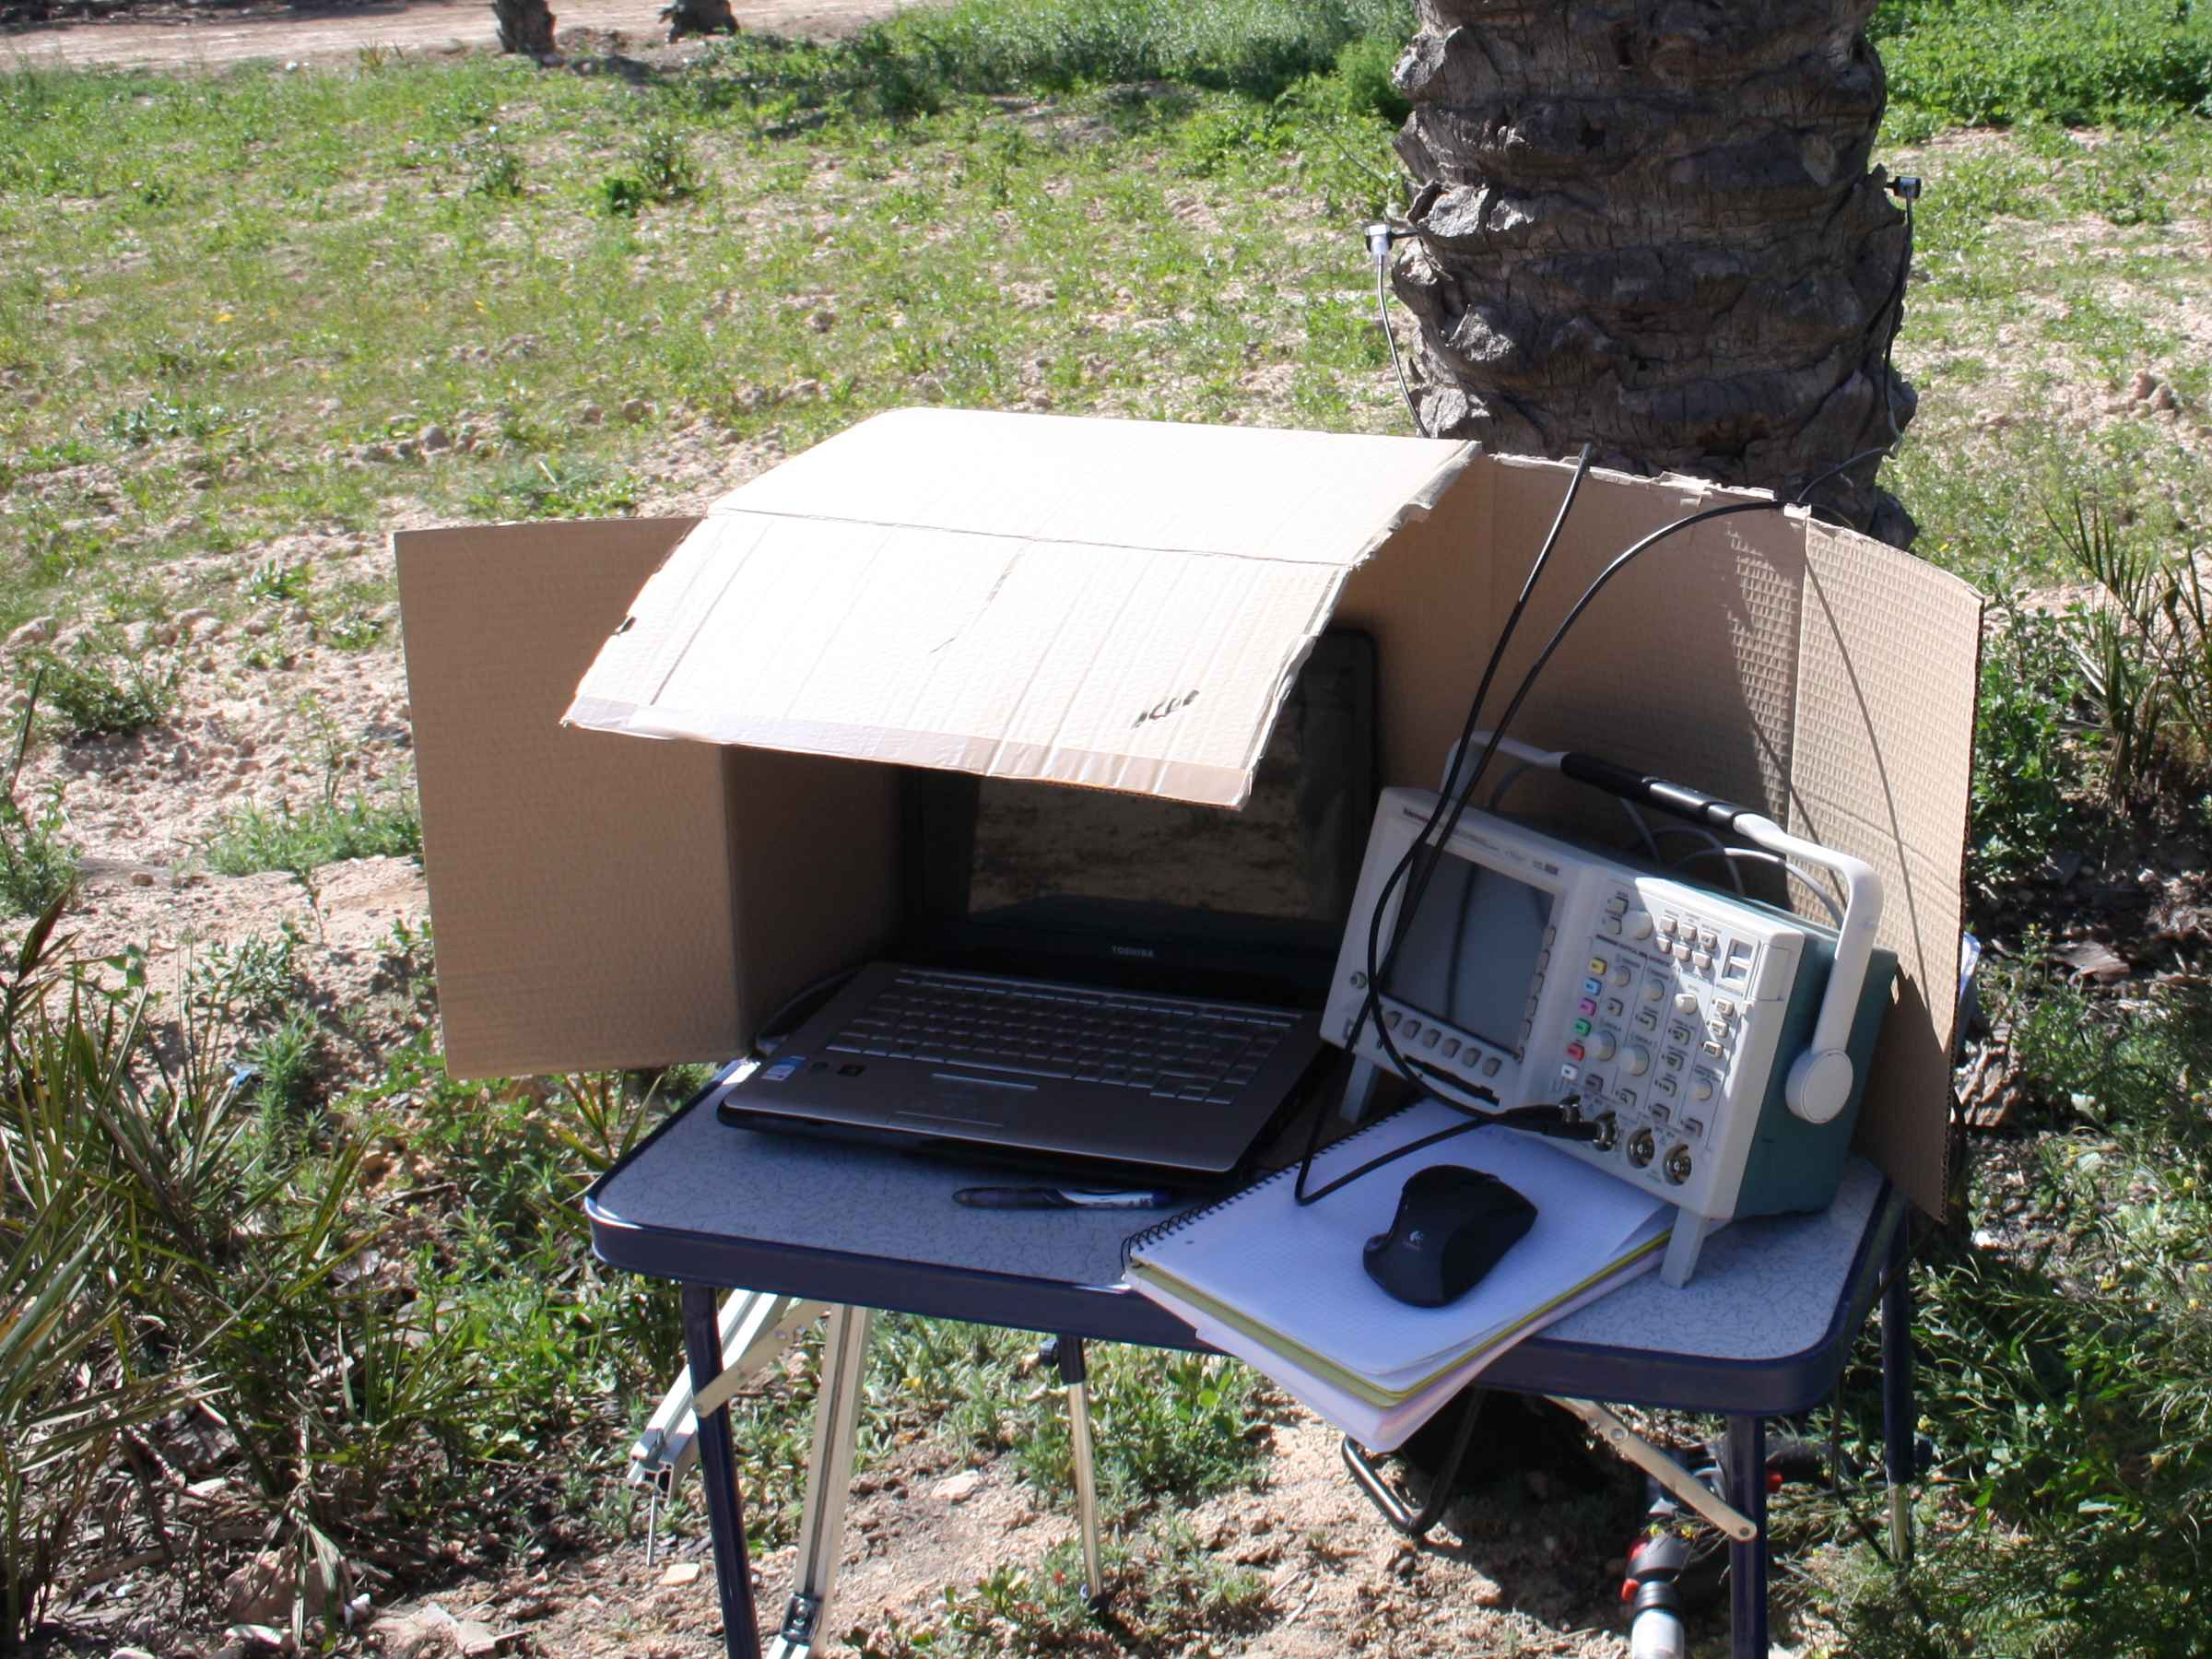
\includegraphics{gis-pfc-ch6-01.jpg}
    \end{center}
    \caption[Equipo utilizado durante los ensayos]{Equipo utilizado durante
    los ensayos realizados.}
    \label{fig:equipment}
\end{figure}


\subsection{Transductores de impacto}

Los transductores de impacto o sondas piezoeléctricas de impacto son
transductores específicos para aplicaciones que implican la realización de
ensayos no destructivos en ejemplares de árboles in vivo. En este caso
resultan útiles también para evaluar las propiedades de las palmeras puesto
que éstas crecen de forma arborescente. Están formados por un punzón que se
inserta levemente en el tallo del ejemplar sometido a estudio sin que ello
le cause ningún daño, quedando la sonda bien sujeta. El punzón canaliza
eficazmente la onda acústica transmitida al tronco del árbol, es capaz
igualmente de capturar la máxima energía que proviene del impulso
ultrasónico una vez éste se ha propagado por el medio. Los transductores de
impacto cuentan también con una cabeza metálica que recubre el propio
transductor, esta cabeza metálica está diseñada para poder amartillarse y
es capaz simultáneamente de resistir el impacto, protegiendo la parte
activa de la sonda, y de transmitir toda la fuerza del golpe al árbol por
medio de la onda acústica. Finalmente las sondas de impacto disponen de un
cable coaxial por medio del cual transmiten la señal eléctrica que generan
al sistema de medida; dicho cable está terminado en un conector de rosca
compatible con osciloscopios.

\begin{figure}
    \begin{center}
	\subfloat[Dispositivo empleado como actuador de
	    ultrasonidos][Dispositivo actuador.]
	    {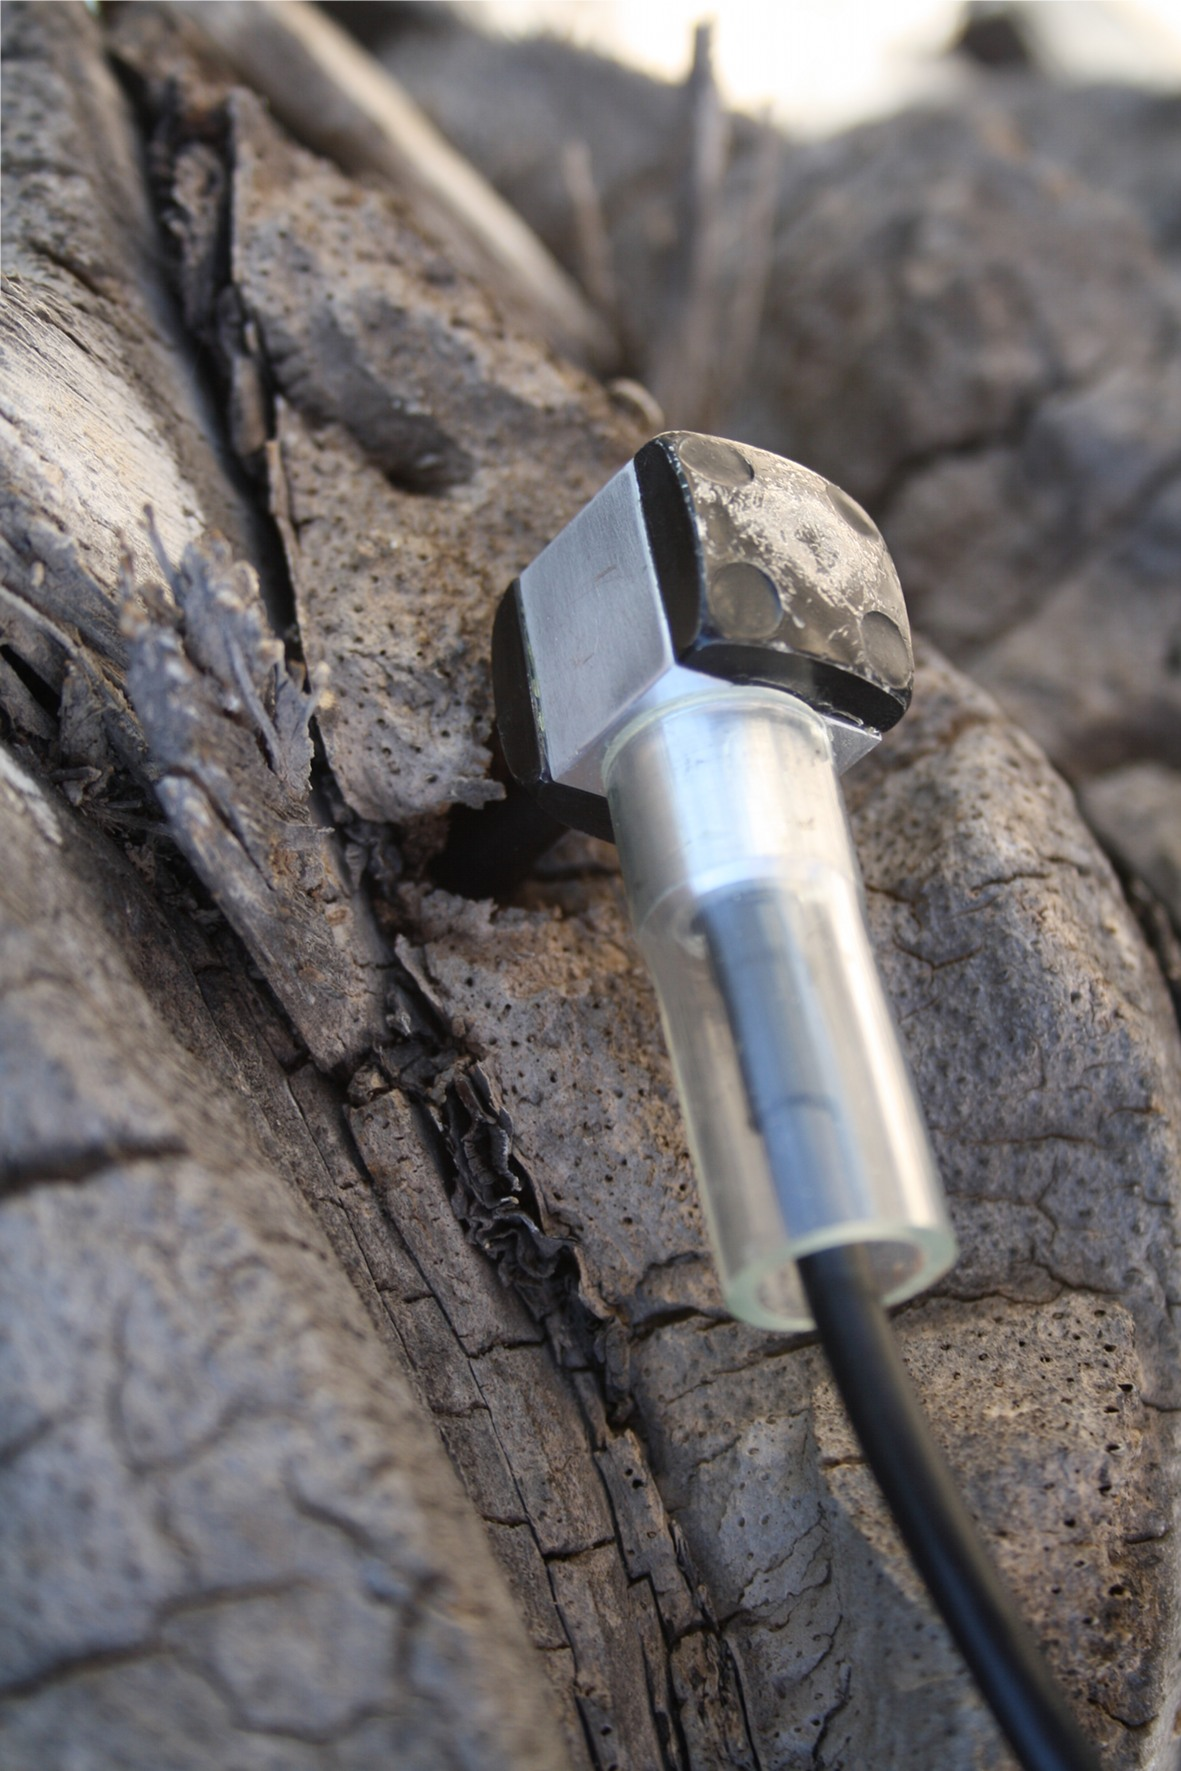
\includegraphics{gis-pfc-ch6-02.jpg}}
	    \qquad
	\subfloat[Dispositivo empleado como sensor de
	    ultrasonidos][Dispositivo sensor]
	    {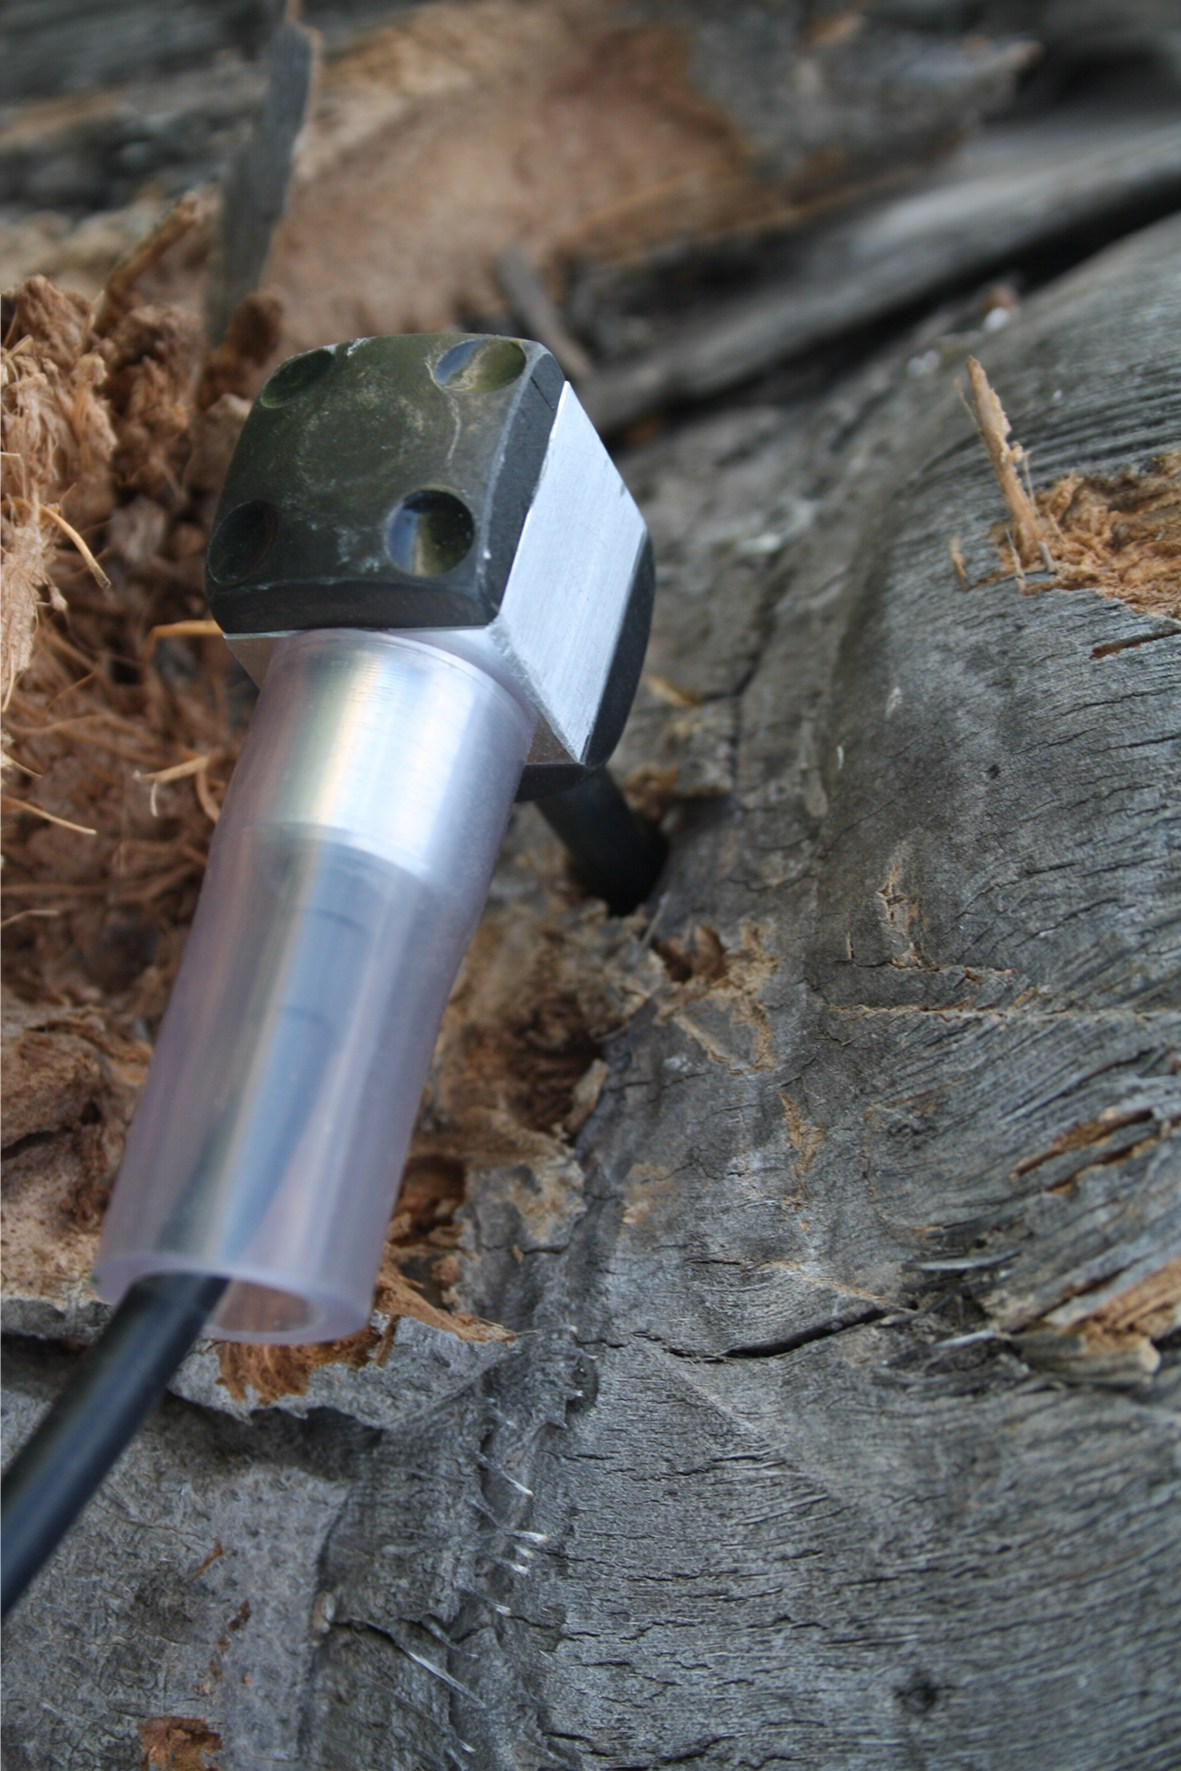
\includegraphics{gis-pfc-ch6-03.jpg}}
    \end{center}
    \caption[Transductores de impacto utilizados durante los
    ensayos]{Imágenes de los transductores tomadas durante la realización
    de los ensayos. Se aprecia la diferencia entre el transductor utilizado
    como actuador y el que se utiliza como sensor al observar las marcas
    que deja el martillo en la cabeza metálica del primero.}
    \label{fig:transducers}
\end{figure}

Este tipo de transductor puede utilizarse indistintamente como actuador o
como sensor ya que es la estructura metálica externa del transductor la
que, al recibir el golpe del martillo, genera y transmite la onda acústica.
Por su parte, el componente activo de la sonda realiza la transformación de
onda de presión a onda eléctrica y únicamente en este sentido\footnote{Es
fácil observar que el sentido de la conversión es único, puesto que la
sonda coaxial que conecta el sensor con el osciloscopio únicamente
transmite información en forma de señal eléctrica y únicamente en el
sentido que va del transductor al osciloscopio. Además es bien sabido que
los osciloscopios no generan señal alguna por sus canales de medida.}. Si
el transductor actúa como sensor envía una señal eléctrica correspondiente
con la onda acústica recibida, por el contrario, si sirve como actuador
transmite la correspondiente a la onda transmitida; de ese modo es fácil
registrar ambas señales.

En concreto los transductores utilizados en este proyecto fin de carrera
han sido fabricados por el fabricante húngaro de equipos para la
realización de pruebas no invasivas
\href{http://www.fakopp.com/site/piezo}{fakopp}. Se trata de transductores que,
pese a estar diseñados para resistir el impacto de un martillo, ofrecen una
buena relación señal a ruido. Funcionan a una frecuencia de resonancia
propia de 45 kHz (es menester recordar que la banda de actuación de los
ultrasonidos parte de los 20 kHz y llega a los 1000 MHz, por lo que una
frecuencia de 45 kHz es en este contexto una frecuencia relativamente
baja) adecuada para el tipo de ensayos que se desea realizar en este
apartado del proyecto.


\subsection{Resto de equipo utilizado}

A parte de los transductores, el equipo utilizado para la realización de
ensayos no destructivos en palmeras in vivo no difiere mucho del que
comúnmente se utiliza para ejecutar pruebas similares.

Para la adquisición de datos se ha utilizado un osciloscopio de laboratorio
conectado por medio de un enlace de red, en una comunicación par a par, a
un \sig{pc}. El propósito del \sig{pc} es el de almacenar las muestras que
se obtienen con el osciloscopio. Al emplear pulsos acústicos es preciso
configurar el disparo del osciloscopio apropiadamente (en base a la señal
transmitida), de lo contrario los pulsos transmitido y recibido salen
rápidamente de pantalla y apenas se perciben.

Para preparar el árbol para las pruebas se ha precisado de un taladro y una
azadilla. Las palmeras disponen de una corteza muy resistente y difícil de
penetrar formada por los restos de antiguas ramas que quedan después de que
éstas se poden. Al estar formada por madera <<muerta>>, la corteza de la
palmera puede alterar los resultados de las pruebas por lo que antes de
fijar los transductores es necesario limpiar una pequeña zona de la planta
y proporcionar acceso al verdadero tallo.

Los dispositivos electrónicos utilizados, así como el taladro mecánico,
precisan de suministro eléctrico para funcionar. Al realizarse las pruebas
en terreno abierto no existe otra alternativa que la de alimentar estos
instrumentos por medio de una batería. Sin embargo, las baterías generan
una tensión continua que no es compatible con los requisitos de aparatos
diseñados para proveerse de la red eléctrica, por lo tanto ha sido
necesario también el uso de un transformador de continua a alterna junto
con la batería. Además para gozar de cierta movilidad durante las pruebas
se ha hecho uso de una alargadera común.

El procedimiento para determinar la velocidad de propagación de la onda
ultrasónica comprende averiguar el tiempo de vuelo de la onda y medir el
espesor de la muestra, dividiendo estas dos magnitudes se obtiene la
velocidad de propagación. Medir el espesor del tallo de una palmera se hace
difícil con una cinta métrica, por no decir que las medidas tomadas son
poco precisas. Por este motivo para la realización de ensayos en los que se
desea registrar también el espesor del espécimen evaluado se fabrica un
calibre apropiado. El calibre de factura propia, mostrado en la
\cref{fig:calibre}, permite determinar de un modo significativamente más
sencillo y exacto el grosor del tallo.

\begin{figure}
    \begin{center}
	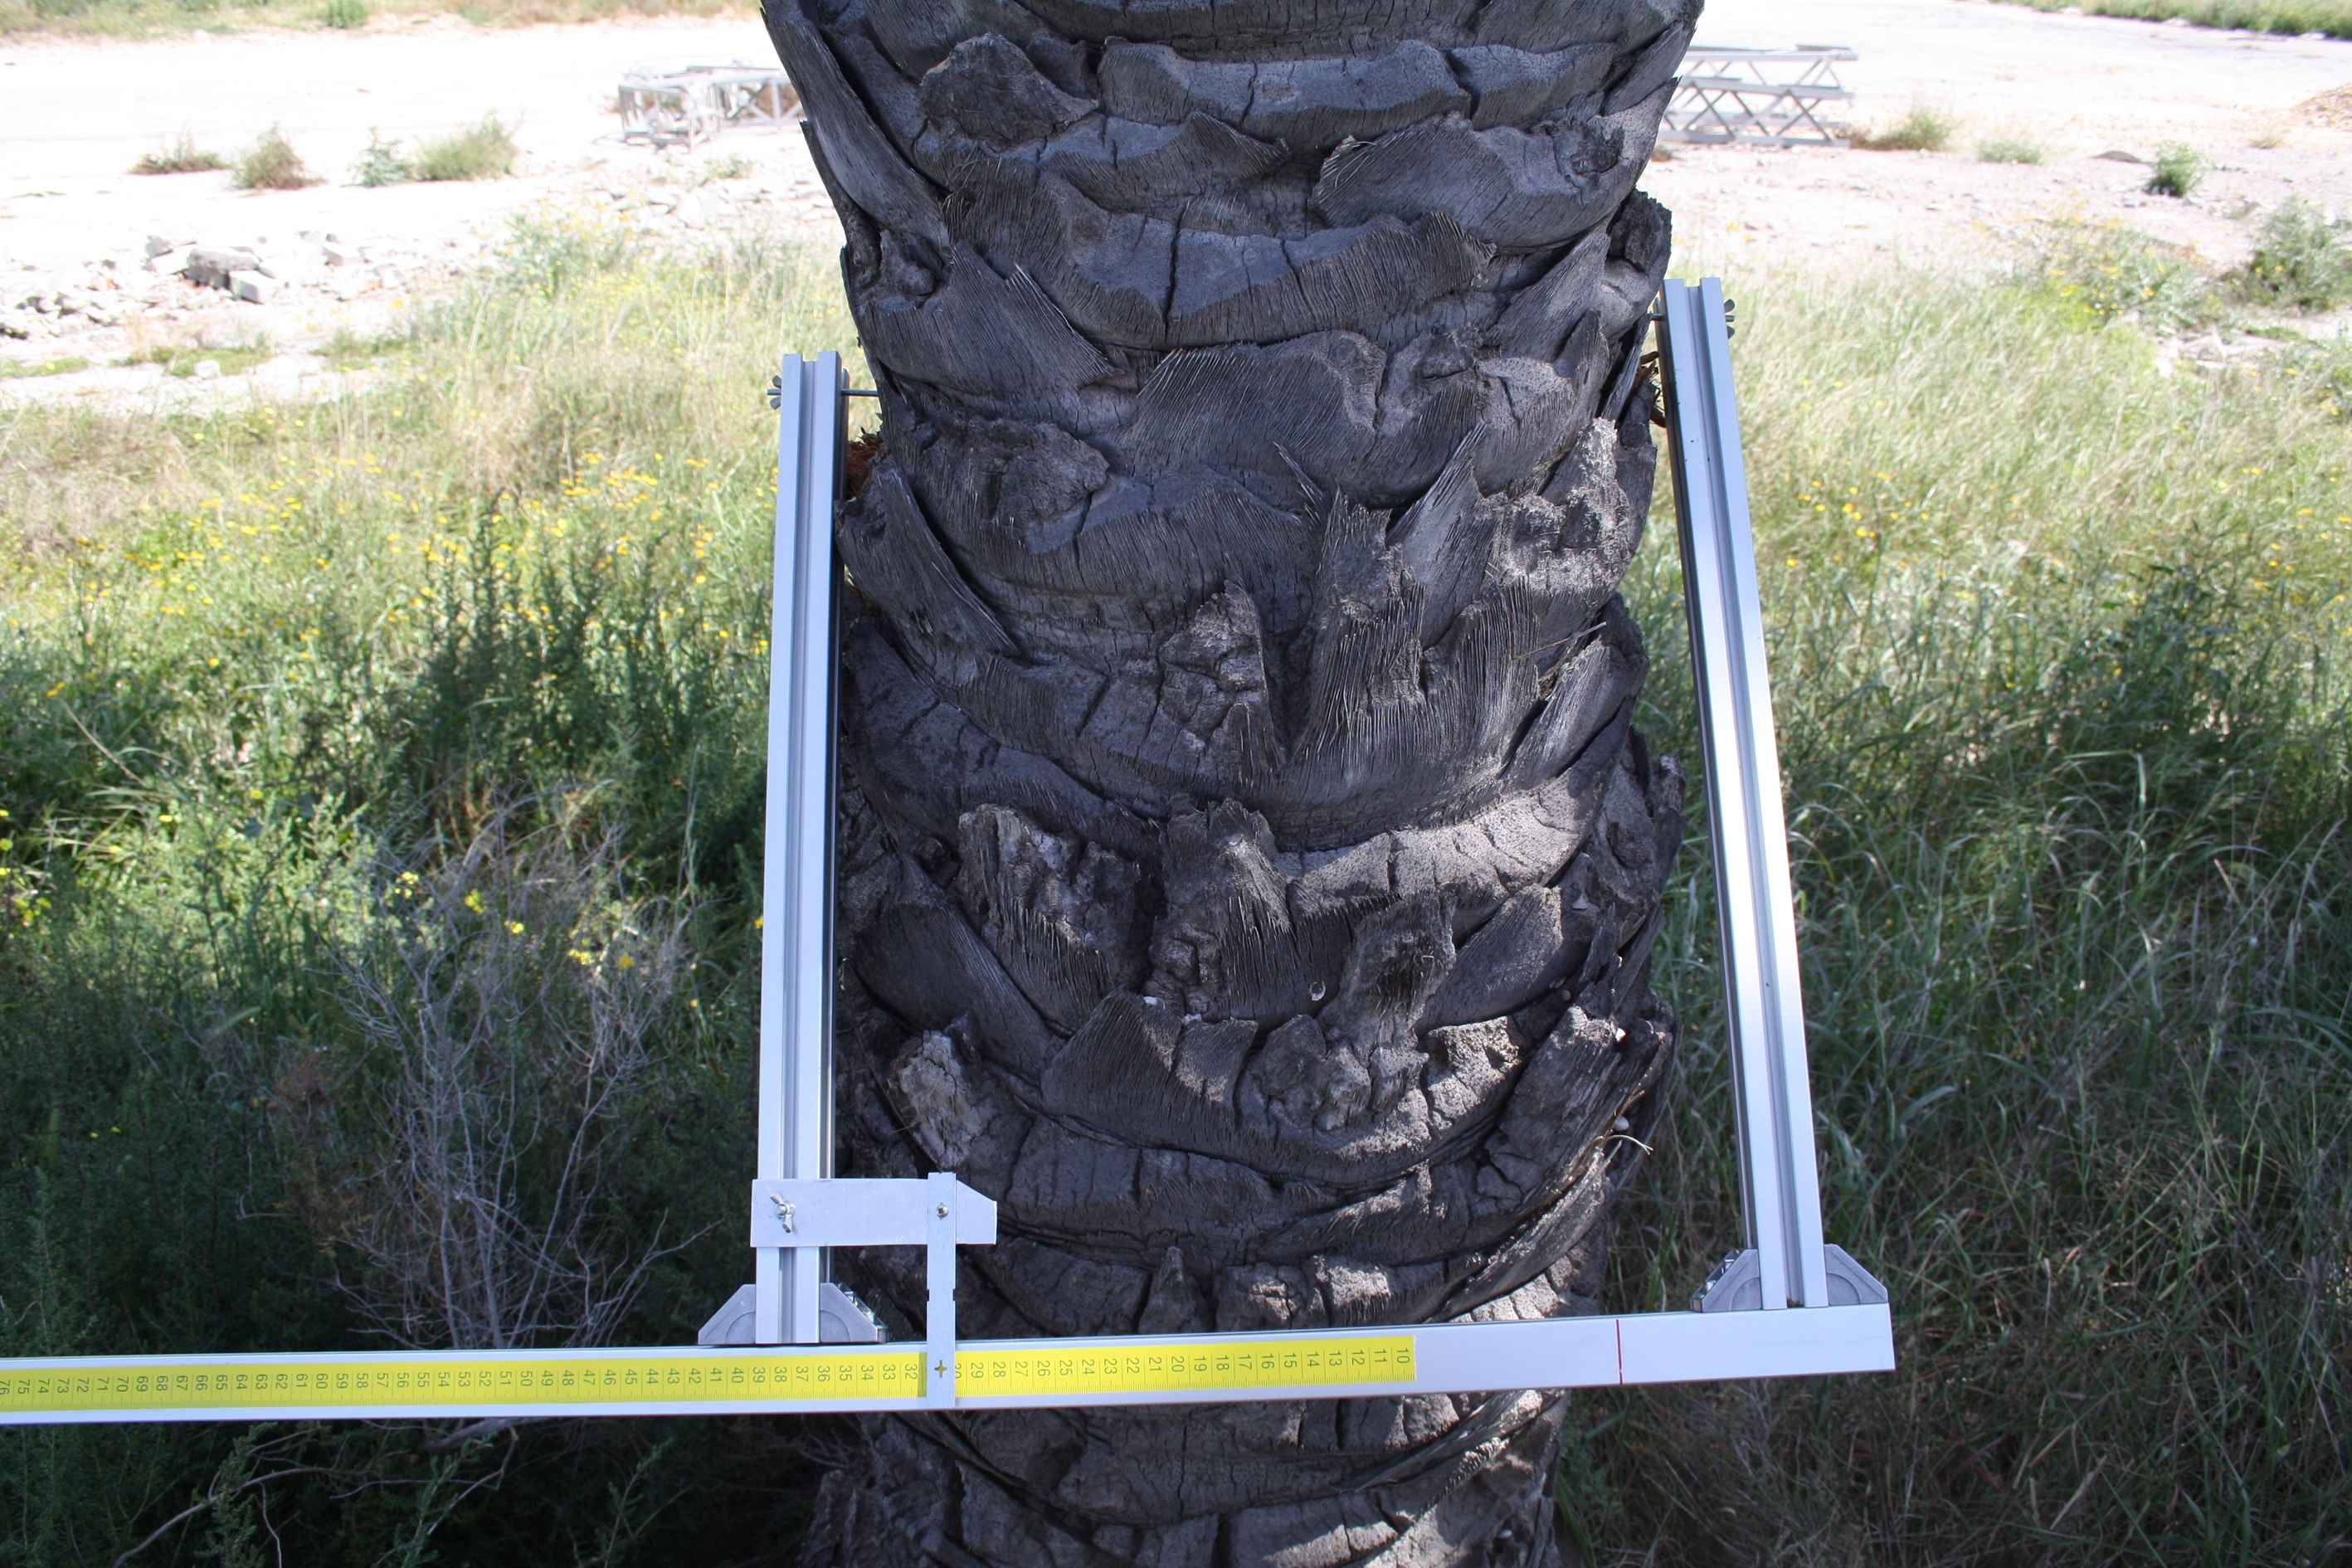
\includegraphics{gis-pfc-ch6-04.jpg}
    \end{center}
    \caption[Calibre en los ensayos]{Calibre construido a propósito de los
    ensayos realizados. Permite evaluar fácilmente y con mayor precisión el
    espesor de la muestra.}
    \label{fig:calibre}
\end{figure}

Para terminar se exponen aquí el resto de elementos incluidos en el equipo
utilizado, se trata principalmente de instrumentos utilizados para
registrar las dimensiones u otras características de las muestras: una
cinta métrica, una referencia y una cámara de fotos (para obtener un valor
aproximado de la altura total de la palmera comparando en las fotografías
realizadas la altura de las marcas situadas a distintos niveles en la
referencia, que es conocida, con la del ejemplar), un martillo para
percutir el sensor y en último lugar, pero no por ello menos importante,
bolígrafo y papel para realizar anotaciones.


\section{Metodología seguida durante las pruebas}

Las pruebas realizadas persiguen demostrar que existe una relación entre
los distintos parámetros de la señal recibida y las características del
medio en que se propaga. Si así fuese quedaría justificado un estudio más
ambicioso cuyo objetivo sería el de determinar de forma inequívoca dicha
relación. Los parámetros que se pretende evaluar para intentar dictaminar
que dicha relación en efecto existe son los listados a continuación:

\begin{itemize}
    \item Amplitud de la señal, para determinar en que medida se ha visto
	atenuada la onda sónica al propagarse.
    \item Aparición de dispersión, se evalúa si hay signos visibles del
	efecto de la dispersión en la onda recibida.
    \item Velocidad de propagación, el cociente del diámetro del ejemplar y
	el tiempo de vuelo ayudan a determinar la velocidad de propagación
	de la onda.
    \item Desplazamiento en frecuencia, se observa la posición del máximo
	del espectro frecuencial de la onda ultrasónica.
    \item Curva de atenuación, o forma de la señal, se evalúa si la caída
	de la señal es más o menos suave o abrupta.
    \item Aparición de secundarios, debidos a efectos varios como la
	propagación de onda superficial.
\end{itemize}

Estos parámetros se evalúan en los resultados recogidos al realizar
diferentes ensayos en muestras de distintos tipos, como son: palmeras
sanas, se toman muestras de palmeras ubicadas en distintas localizaciones,
realizando ensayos en ejemplares pertenecientes a múltiples variedades y
que presentan asimismo características variadas como grosor o tipo de
corteza; además se evalúa palmeras muertas o ejemplares que aparentan un
mal estado de salud, eucaliptos, pinos y, finalmente, postes de telefonía.
De ese modo es posible realizar una comparación posterior para tratar de
identificar una relación entre los parámetros estimados y las condiciones o
tipo de la muestra.

El lector ha de notar que no es posible extraer resultados válidos de
muestras de palmera en laboratorio. Ello es debido a que el tallo de la
palmera pierde sus propiedades originales cuando el ejemplar muere.
Mientras vive una palmera intercambia nutrientes y agua entre su copa y sus
partes basales a través de vasos que integran su tallo, principalmente
utilizando un mecanismo basado en la capilaridad. Al morir el individuo
este proceso se detiene y el tallo va perdiendo su composición húmeda
regularmente hasta que finalmente se seca por completo. Debido a esta otra
singularidad que presentan las palmeras, los resultados obtenidos en
muestras extraídas de los restos de un ejemplar no son confiables y no
aportan información válida para la finalidad de este estudio. Es por ello
por lo que los ensayos que aquí se han realizado en ejemplares, palmeras,
in vivo.

La relación entre las propiedades de la madera de palmera y los parámetros
de la señal evaluados es, como se ha afirmado anteriormente, desconocida;
pero no sólo eso, el modo en que las condiciones externas influyen en el
medio es también desconocido. Por último cabe destacar aquí, en parte para
el posterior entendimiento de las conclusiones y resultados expuestos en
este documento que: debido al motivo que se ha manifestado, carece de
sentido comparar los datos obtenidos de las ondas recibidas al realizar
ensayos en las distintas muestras siempre que no se haga en el contexto
---esto es, mirando también las características--- de la onda que parte del
emisor durante la realización de cada prueba.


\subsection{Procedimiento de medida}

Durante la realización de las pruebas se ha seguido un procedimiento
concreto con el objetivo de tomar las medidas de una forma ordenada. El
conjunto de pasos de que consta dicho procedimiento se expone aquí de
forma resumida.

\begin{enumerate}
    \item En primer lugar se ha de trasladar el equipo a las proximidades
	del ejemplar en el van a realizarse las medidas.
    \item Después se asienta una mesa (u otro soporte) y se dispone el
	equipo para la toma de muestras.
    \item Se conecta el transformador a la batería, la alargadera al
	transformador y el resto de equipos a las tomas de la alargadera.
    \item Se realiza la limpieza de la zona de inserción de las sondas con
	ayuda del taladro y la azadilla.
    \item Se mide el espesor del ejemplar y la altura del tallo a la que se
	van a realizar los ensayos y se anotan en la libreta.
    \item Se toma una fotografía del ejemplar situando la referencia en las
	proximidades.
    \item Se encienden los equipos electrónicos y se insertan los punzones
	de las sondas en el tallo del ejemplar.
    \item Por último se toman las medidas. Para ello, mientras una persona
	golpea el actuador la otra verifica que los ajustes del
	osciloscopio son correctos y realiza la transferencia de datos
	desde el osciloscopio hasta el \sig{pc}. Se recogen de entre cinco
	a siete muestras por ejemplar.
\end{enumerate}

Se muestran a continuación las \cref{fig:testheight,fig:testequipment}, son
dos fotografías tomadas durante la ejecución de los ensayos. Estas
fotografías complementan la descripción que se ha hecho de los pasos que
comprende el procedimiento de toma de medida, de modo que el lector pueda
comprender mejor como se han realizado los ensayos. La primera de las
figuras muestra una palmera que, a juzgar por el tamaño que ocupa en la
figura en comparación con las dimensiones de la referencia se calcula que
debe medir unos $5.5$ metros altura aproximadamente. La segunda muestra a
su vez una palmera de medidas similares y parte del equipo utilizado
dispuesto para la toma de muestras.

\begin{figure}
    \begin{center}
	\subfloat[Fotografía que muestra una palmera de unos $5.5$ m de
	    alto][Palmera alta.]{
		\label{fig:testheight}
		\begin{minipage}[c]{.425\textwidth}
		    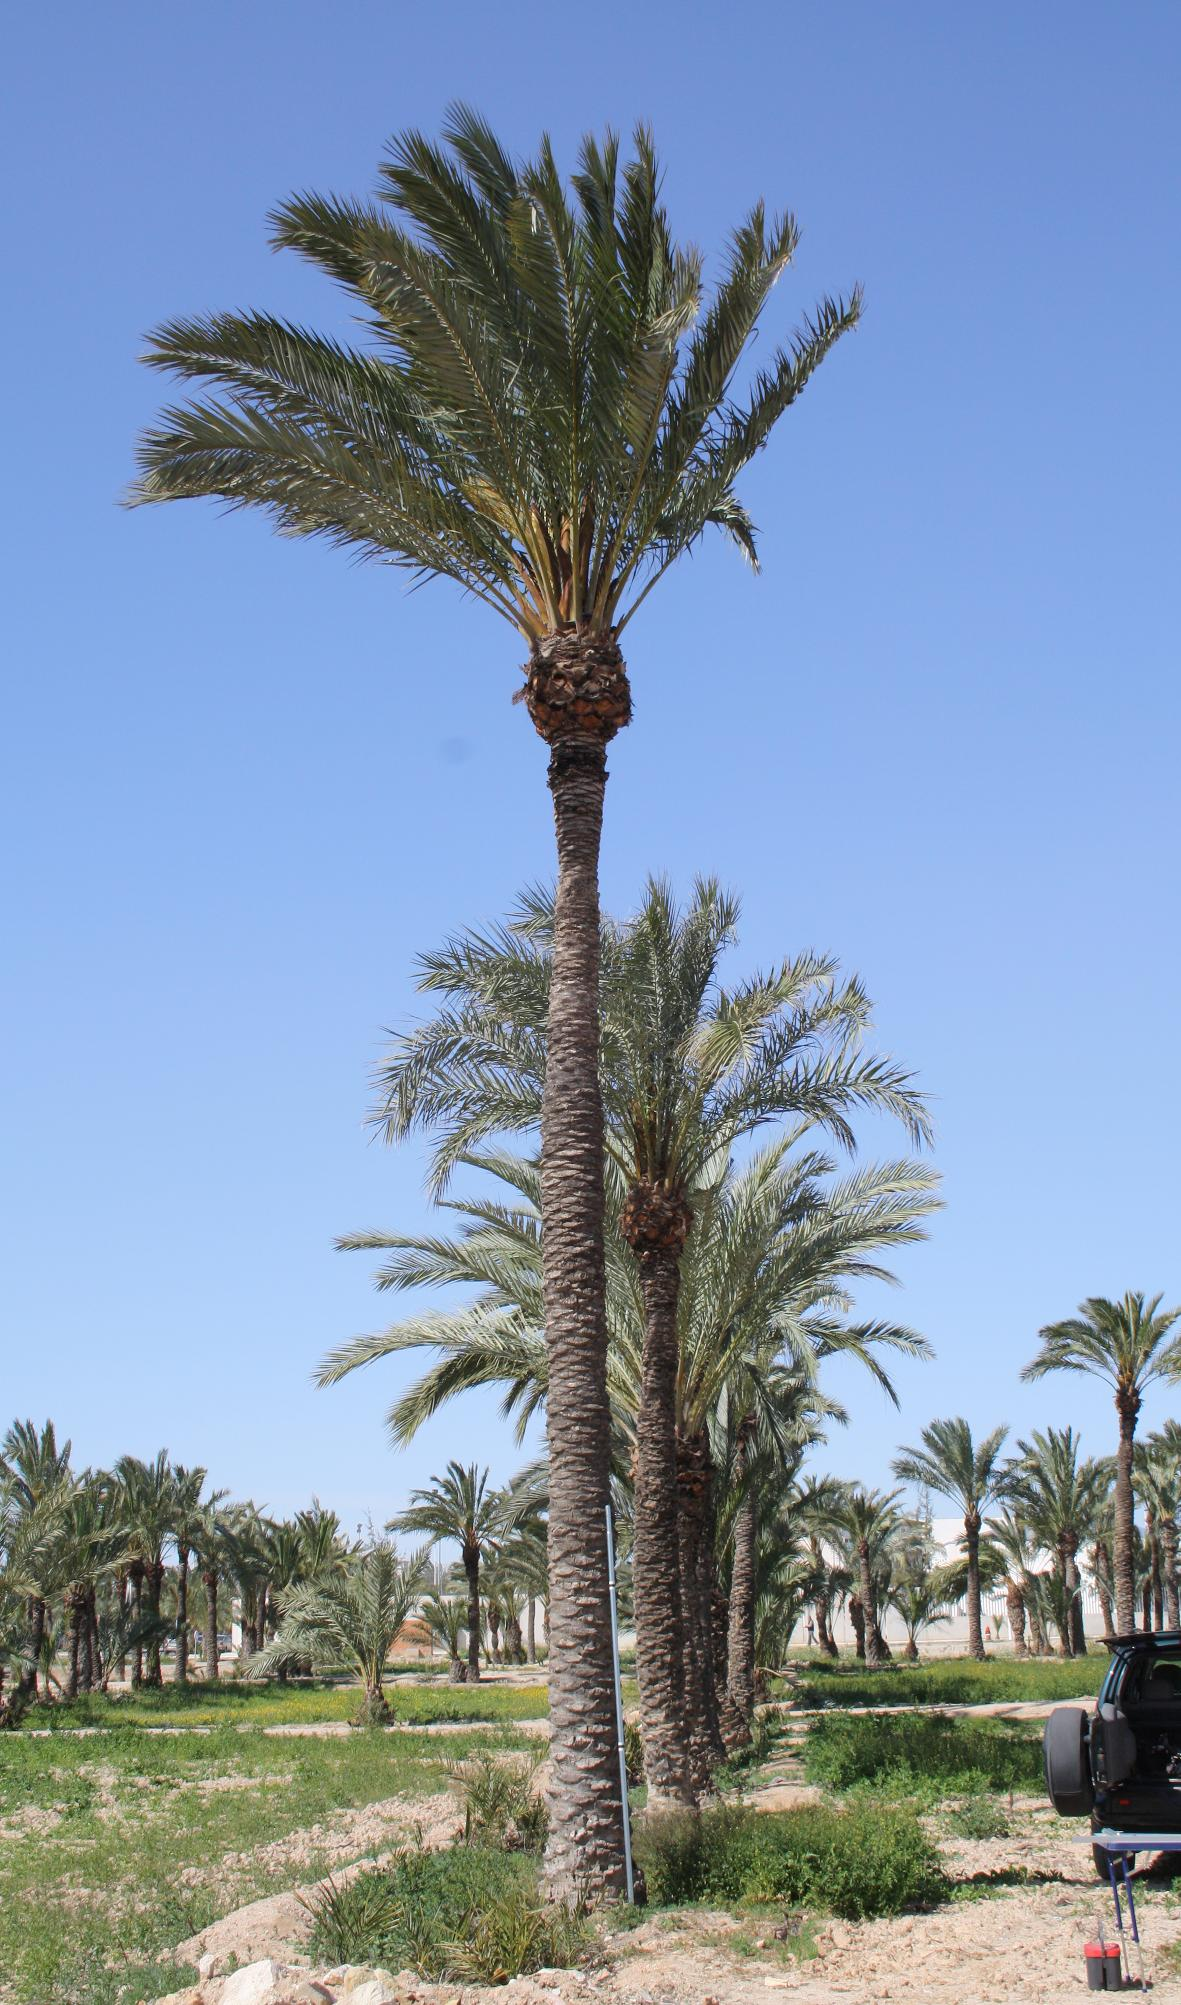
\includegraphics{gis-pfc-ch6-05.jpg}
		\end{minipage}}
	\subfloat[Fotografía en la que puede apreciarse parte del equipo
	    utilizado.][Palmera mediana.]{
		\label{fig:testequipment}
		\begin{minipage}[c]{.425\textwidth}
		    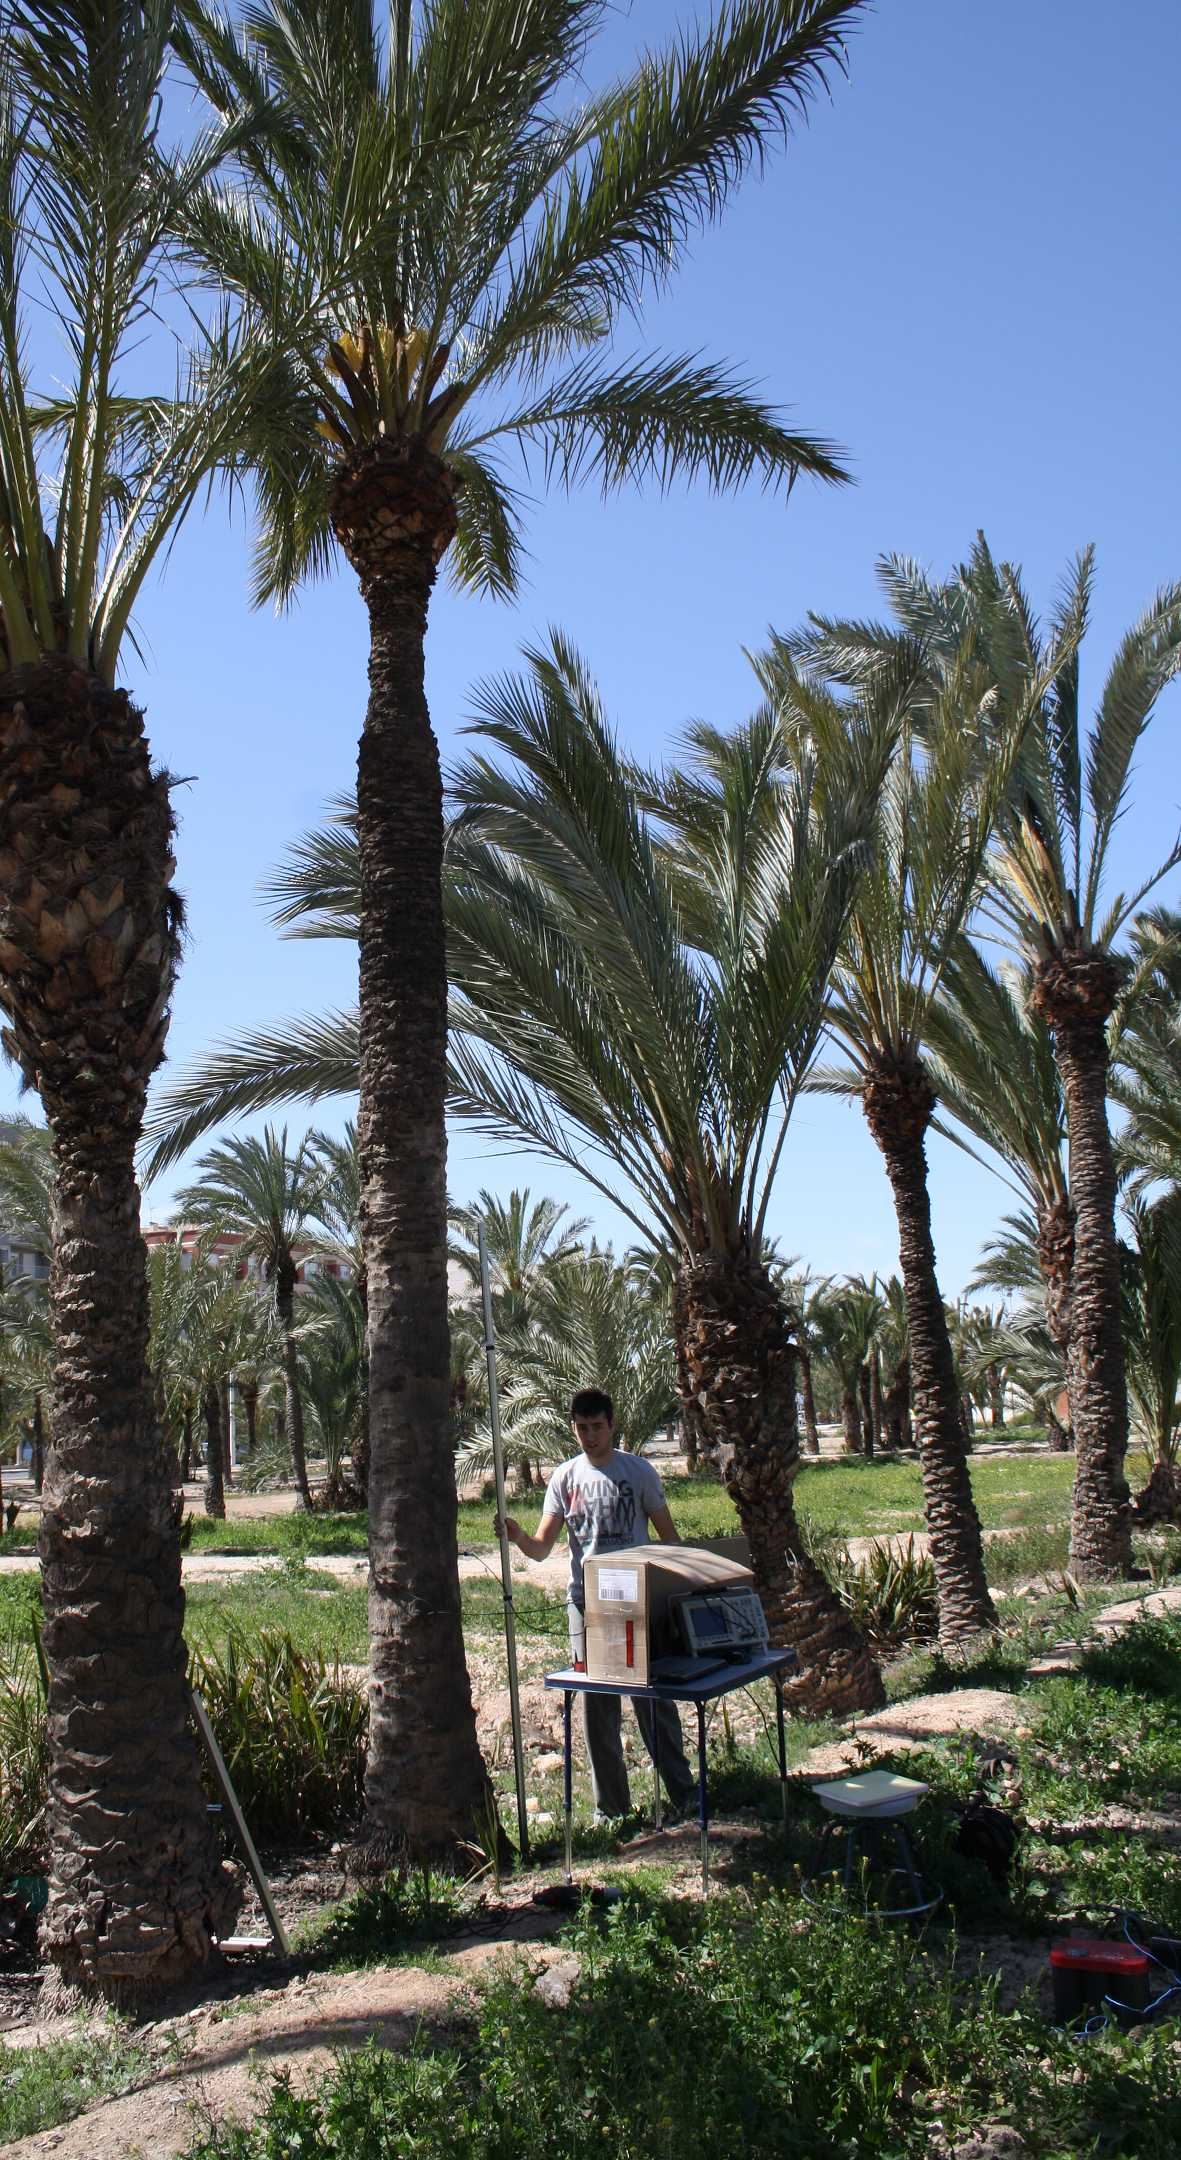
\includegraphics{gis-pfc-ch6-06.jpg}
		\end{minipage}}
		\end{center}
    \caption[Fotografías tomadas durante la realización de los
    ensayos]{Fotografías tomadas durante la realización de los ensayos.}
    \label{fig:tests}
\end{figure}


\subsubsection{Inconvenientes surgidos durante la toma de medidas}

El procedimiento de medida ha resultado tedioso y complejo no sólo por el
hecho de que el procedimiento que ha de ejecutarse para tomar las muestras
es largo, complejo y fatigoso; si no también debido a los siguientes
motivos.

En primer lugar, al realizarse medidas de campo, es preciso trasladarse a
la ubicación en la que se encuentra localizada la muestra para poder
realizar las medidas. Las muestras potenciales, por su naturaleza, se
encuentran en terreno de difícil acceso como zanjas o huertos, a los que es
preciso trasladar el voluminoso equipo para poder realizar las medidas. En
cada ocasión se ha de desplazar el equipo hasta las proximidades de la
muestra y después dicho equipo debe disponerse de modo que el ensayo pueda
ser realizado. Tarea que no siempre es fácil, debido ---como se ha dicho---
a la naturaleza del terreno que frecuentemente resulta irregular y
accidentado, con lo cual la simple acción de asentar una mesa se convierte
en complicada.

Por otro lado, gran parte del equipo utilizado requiere de alimentación
eléctrica para funcionar, al operar en lugares apartados se ha precisado de
una batería para alimentar los distintos dispositivos utilizados. La
capacidad de la batería es limitada lo que limita la duración de una sesión
de toma de muestras. Además, al agotarse es preciso detener las pruebas
durante el periodo de recarga de la batería, que dura aproximadamente un
día, antes de poder reemprender los ensayos.

A todo ello debe añadirse que tanto el director como el proyectista en este
proyecto fin de carrera desconocían previamente a los ensayos el manejo de
los transductores de impacto que se han empleado para la realización de las
pruebas, lo cual ha dificultado, más aún si cabe, la ejecución de los
ensayos.


\section{Resultados obtenidos}

Tras finalizar el proceso de medida se disponía de 420 muestras (210
correspondientes a ondas acústicas transmitidas y otras 210
correspondientes a las respectivas ondas recibidas).

tengo que decir que he procesado con cuidado las muestras y he creado
aplicaciones en matlab que me permitiesen observar los datos que voy a
exponer ahora.
